\documentclass[a4paper,12pt]{article}
\usepackage[margin=0.8 in]{geometry}

\usepackage[T2A]{fontenc}			% кодировка
\usepackage[utf8]{inputenc}			% кодировка исходного текста
\usepackage[english,russian]{babel}	% локализация и переносы
\usepackage{graphicx}                % Математика
\usepackage{amsmath,amsfonts,amssymb,amsthm,mathtools} 
\usepackage{mathtext}
\usepackage[T2A]{fontenc}
\usepackage[utf8]{inputenc}

\usepackage{wasysym}

%Заговолок
\author{Бичина Марина 
группа Б04-005 1 курса ФЭФМ}
\title{}
\date{}


\begin{document} % начало документа

\begin{center}
\begin{Large}
{Бичина Марина Б04-005, Лабораторная работа №.3.5.1}
\end{Large}
\end{center}
\paragraph{Цель работы:} 
\begin{enumerate}
\itemsep0em
\item Измерить вольт-амперную тлеющего характеристику тлеющего разряда 
\item Измерить зондовые характеристики при разных токах разряда и изучить таким образом свойства плазмы (концентрацию и температуру электронов в плазме, степень ионизации,  плазменную частоту и дебаевский радиус экранирования)
\end{enumerate}
\paragraph{Оборудование:}
\begin{enumerate}
\itemsep0em
\item Стеклянная газоразрядная трубка, наполненная неоном
\item Высоковольтный источник питания 
\item Источник питания постоянного тока
\item Делитель напряжения
\item Потенциометр
\item Амперметры
\item Вольтметры
\item Переключатели
\end{enumerate}


\paragraph{Теоретическая справка:}
\paragraph{}

\paragraph{Описание установки:}
\paragraph{}
\begin{center}
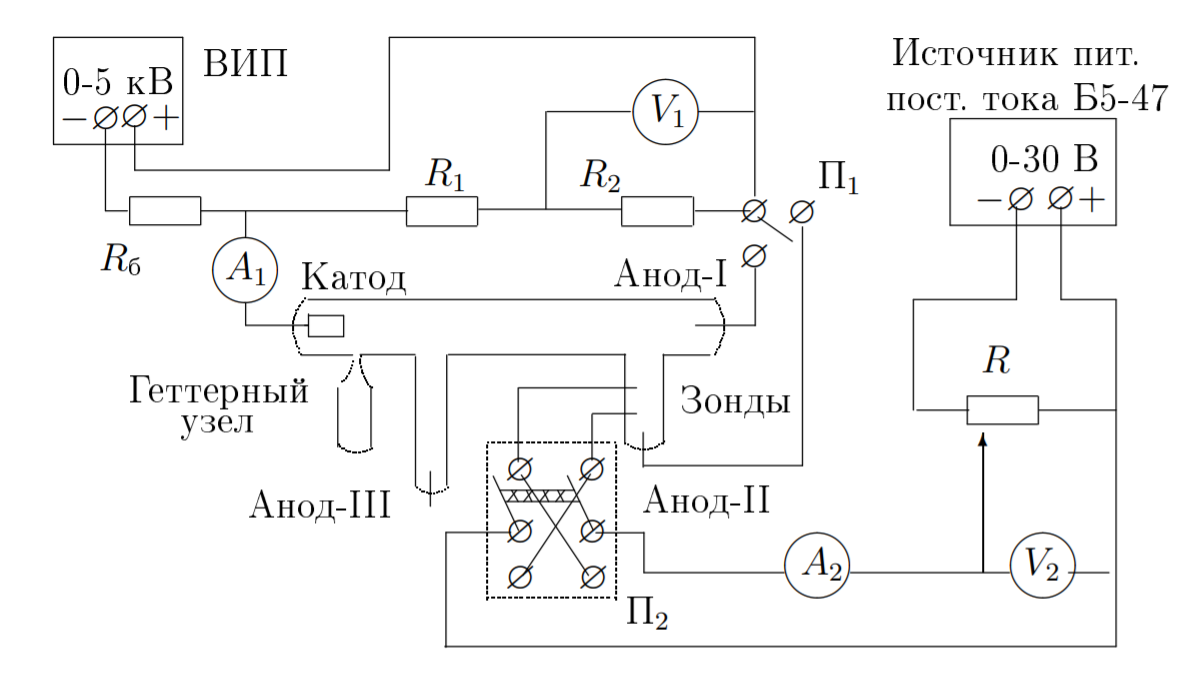
\includegraphics[scale=0.55]{setup.png}
\end{center}
\setlength{\parindent}{1.5 cm}
	Стеклянная газоразрядная трубка имеет холодный полый катод, три анода и \textit{геттерный} узел. Трубка наполнена изотопом неона $^2_2$Ne при давлении 2 мм рт. ст. Катод и один из анодов (I и II) с помощью переключателя $\Pi_1$ подключается через балластный резистор $R_\text{б}$ ($\approx 450$ кОм) к регулируемому ВИП с выходным напряжением до 5 кВ.\\
	Зонды изготовлены из молибденовой проволоки диаметром $d = 0.2$ мм и имеют длину $l = 5.2$ мм.

\paragraph{Ход работы:}
\begin{enumerate}
\itemsep0em
\item Рассмотрим ВАХ разряда: для этого по снятым данным построим график
\begin{figure}[h!]
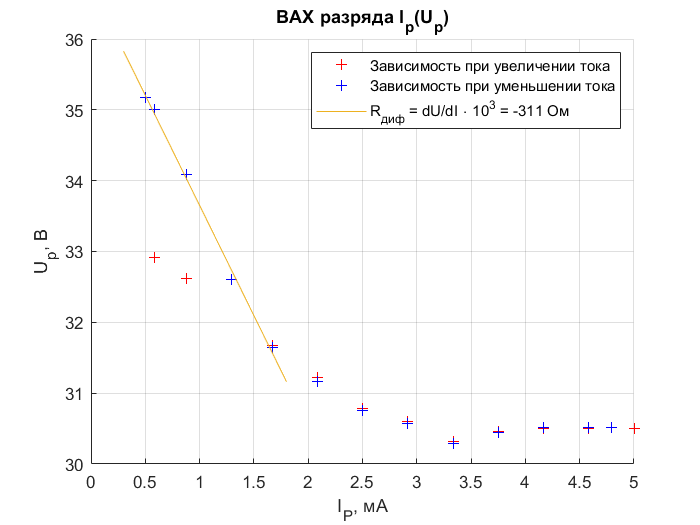
\includegraphics[scale=0.8]{graph_r.png}
\label{razr}
\caption{}
\end{figure}
 
 Далее по наклону прямой найдем максимальное дифференциальное  сопротивление разряда, получим $\dfrac{dU}{dI} = -310 \pm 10 \;\;\text{Ом}$
 
 Дифференциальное сопротивление может быть отрицательным, поскольку возрастание тока приводит к возрастанию концентрации ионов, что приводит к возрастанию
проводимости и понижению напряжения

\begin{figure}[h!]
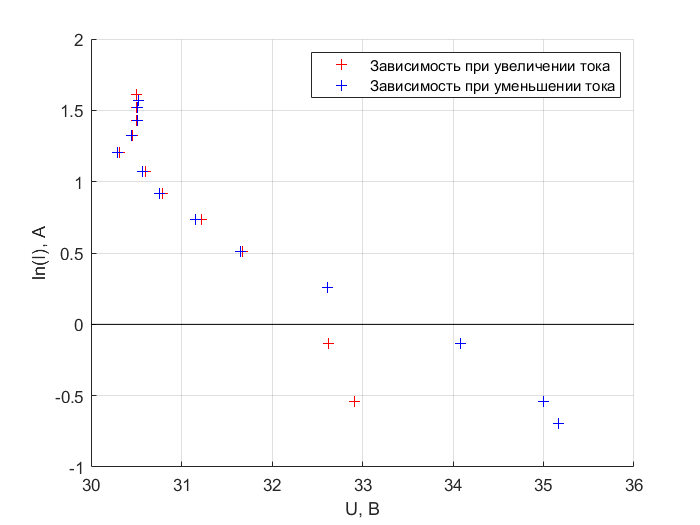
\includegraphics[scale=0.8]{graph_r_log.png}
\label{razr}
\caption{}
\end{figure}
\end{enumerate}
\paragraph{Выводы:}
\begin{enumerate}
\item
\end{enumerate}
\end{document}